%---------------------------------------------------------------------
\begin{frame}{Last class}

    \newbold{Moral hazard}: what is it? why would it be a problem in health insurance?\\
    \vspace{3mm}

    \newbold{Do consumers respond to co-insurance rates in health insurance?}\\
    \only<1>{\vspace{15mm}}
    \only<2>{Yes! Evidence from the RAND health insurance experiment
    \begin{itemize}
        \item Healthcare demand slopes down (elasticity $\approx$ -0.2)
        \item Insurance increases the demand for healthcare
        \item Which care is cut: both ``effective'' and ``rarely effective'' care
        \item Impact on health? None on average but poor adults are hurt
    \end{itemize}
    }

\end{frame}
%---------------------------------------------------------------------
\begin{frame}{What is the impact of health insurance?}

    Insurance reduces the prices faced by patients\\
    $\rightarrow$ increases the demand for healthcare\\
    $\rightarrow$ increases healthcare utilization\\
    \vspace{5mm}

    A trade-off:
    \begin{itemize}
        \item Some healthcare is not very effective for some patients $\rightarrow$ more insurance $\rightarrow$ small gains and high costs
        \item Some healthcare is effective $\rightarrow$ more insurance $\rightarrow$ better health $\rightarrow$ could lead to less spending!
    \end{itemize}

\end{frame}
%---------------------------------------------------------------------
\begin{frame}{What is the impact of health insurance?}

    What do we want to know?
    \begin{align*}
        y_{i} = \pi_0 + \pi_1 \text{INSURANCE}_i + X'_{i} \pi_2 + \epsilon_{i}
    \end{align*}
    where
    \begin{itemize}
        \item $y_i$ is an outcome of interest for individual $i$ (e.g., healthcare utilization, health, financial health)
        \item $\text{INSURANCE}_i$ is whether $i$ has insurance
        \item $X_i$ are observables on individual $i$ (e.g., income, gender, age, etc.)
    \end{itemize}
    \vspace{2mm}

    Parameter of interest? \only<2>{{\color{red} $\pi_1$}}.
    
\end{frame}
%---------------------------------------------------------------------
\begin{frame}{What is the impact of health insurance?}

    What do we want to know?
    \begin{align*}
        y_{i} = \pi_0 + {\color{red} \pi_1} \text{INSURANCE}_i + X'_{i} \pi_2 + \epsilon_{i}
    \end{align*}
    \vspace{3mm}

    Problem? \only<2>{\newbold{Endogeneity of insurance}.\\
    This means that $\text{INSURANCE}_i$ is correlated with $\epsilon_i$:
    \begin{align*}
        cov(\text{INSURANCE}_i, \epsilon_i) \neq 0
    \end{align*}
    Thus OLS estimates of $\pi_1$ will be biased and inconsistent.
    \vspace{4mm}

    What do we do? \textit{We find some exogenous variation in insurance coverage.} How?}

    \only<1>{\vspace{35mm}}

\end{frame}
%---------------------------------------------------------------------
\begin{frame}{The Oregon Health Insurance Experiment}

    Individuals randomly allocated to Medicaid in Oregon
    \begin{itemize}
        \item 2008: Oregon has extra funding for Medicaid
        \begin{itemize}
            \item People have to signup: vastly advertised, 90,000 signed up
            \item Who do you give it to? Random allocation seemed the fairest
            \begin{itemize}
                \item Eight lotteries drew $\sim$ 35,000 names
                \item Eligible + replies: 30\% will be enrolled
                \item Coverage: very low premium and 0\% cost-sharing
                %monthly premium 0 to 20 depending on income
                % no vision and non emergency dental coverage
            \end{itemize}
        \end{itemize}
        $\implies$ \newbold{``natural''} experiment!!
    \end{itemize}
    \vspace{3mm}

    What is the impact of access to \newbold{public insurance} on
    \begin{itemize}
        \item \newbold{Healthcare utilization}: hospital discharge data
        \item \newbold{Health}: mortality records + surveys ($\sim$ 25,000)
        \item \newbold{Financial health}: credit reports (TransUnion's Consumer Credit database)
    \end{itemize}

\end{frame}
%---------------------------------------------------------------------
\begin{frame}{Impact of \textit{winning the lottery}}

    \newbold{Intent-to-treat (ITT)}
    \vspace{-3mm}
    \begin{align*}
        y_{i} = \beta_0 + \beta_1 \text{LOTTERY}_i + X_{i} \beta_2 + V_{i} \beta_3 + \epsilon_{i}
    \end{align*}
    where
    \begin{itemize}
        \item $\text{LOTTERY}_i$ takes value 1 if $i$ won the lottery and 0 otherwise
    \end{itemize}
    \vspace{7mm}

    This is not the impact of health insurance. Why?
    %Some people did get insurance when selected, others not
\end{frame}
%---------------------------------------------------------------------
\begin{frame}{Empirical strategy: instrumental variables (IV)}

    \newbold{Local average treatment effect (LATE)}
    \vspace{-3mm}
    \begin{align*}
        y_{i} = \pi_0 + \pi_1 \text{INSURANCE}_i + X'_{i} \pi_2 + V'_{i} \pi_3 + v_{i}
    \end{align*}
    where
    \begin{itemize}
        \item $\text{INSURANCE}_i$ is insurance coverage (main: ``ever on Medicaid''), \newbold{instrumented} by $\text{LOTTERY}_i$
        %\item \newbold{Exclusion restriction}: potential threats?
        % The lottery has an impact on y only through the gaining of insurance
        % If winning lottery has a direct impact or if makes you more likely to apply to other health programs

        %Reminder: HP for IV (1) random (2) relevance (3) exclusion restriction (4) monotonicity: the instrument induces the same behavior for all
        %[here, being selected makes you more likely to take up for all. No individual is less likely to take up if selected (defier)]
    \end{itemize}
    \vspace{3mm}

    First stage
    \vspace{-3mm}
    \begin{align*}
        \text{INSURANCE}_{i} = \delta_0 + \delta_1 \text{LOTTERY}_i + X'_{i} \delta_2 + V'_{i} \delta_3 + \mu_{i}
    \end{align*}
    % note F-stat = ratio of explained over unexplained variance

    $\implies$ This is called an \newbold{instrumental variable} strategy
\end{frame}
%---------------------------------------------------------------------
\begin{frame}{The impact of public insurance on healthcare utilization}
    \hypertarget{ohie:table}{}
    
        \only<1>{
            \begin{center}
                \vspace{-3mm}
                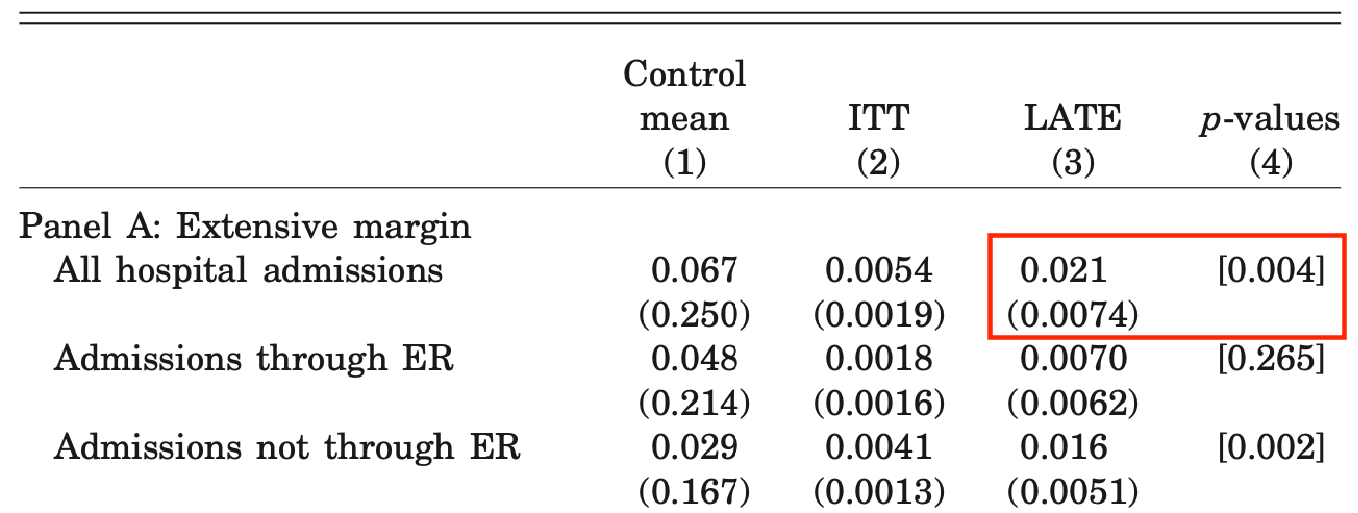
\includegraphics[height=0.6\textheight]{input/ohie_tab4.pdf}
            \end{center}
        }
        \only<2>{
            \begin{center}
                \vspace{-3mm}
                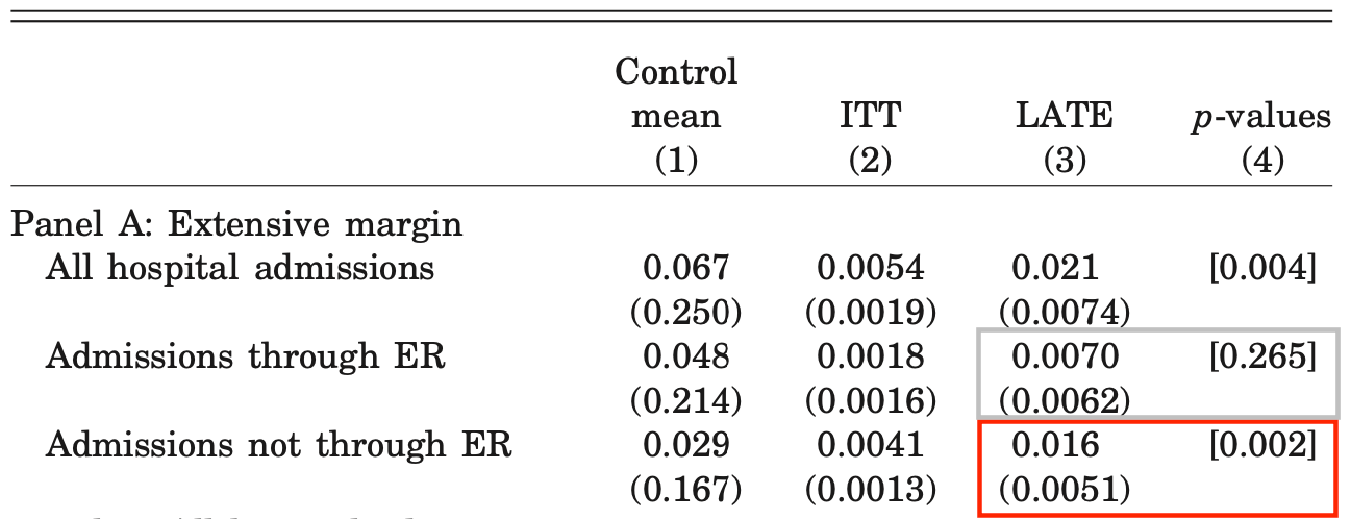
\includegraphics[height=0.6\textheight]{input/ohie_tab4H.pdf}
            \end{center}
        }
        \vspace{-5mm}
        \hyperlink{ohie:ITT}{\beamergotobutton{ITT}}
\end{frame}
%---------------------------------------------------------------------
\begin{frame}{Which kind of utilization? Preventive care}
    
    \begin{center}
        \vspace{-3mm}
        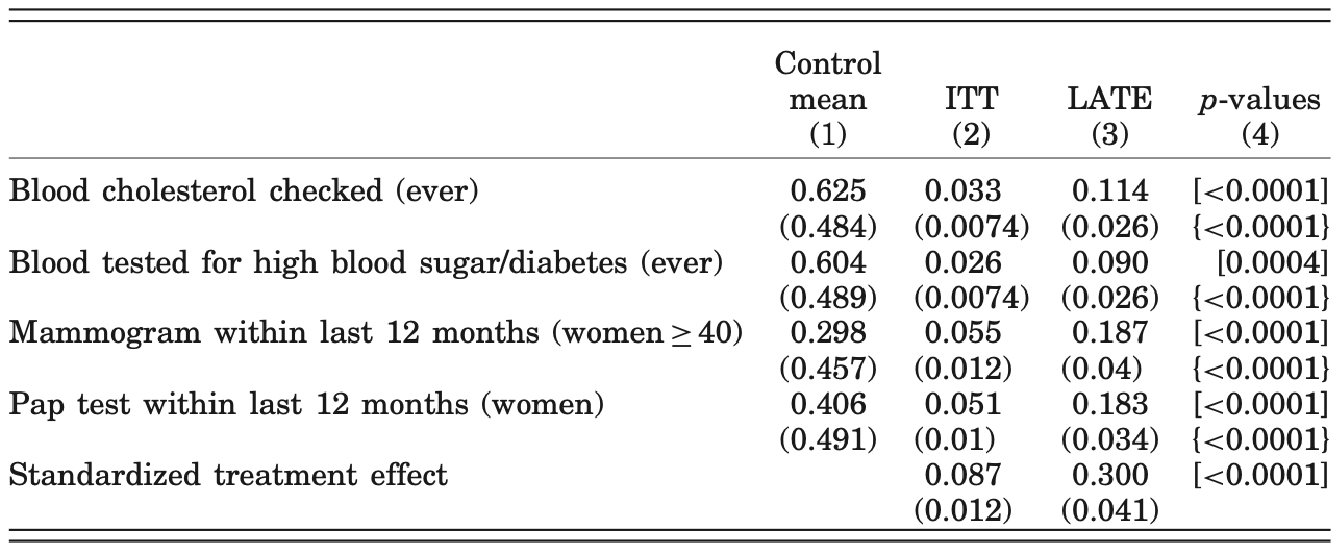
\includegraphics[height=0.6\textheight]{input/ohie_tab6.pdf}
    \end{center}
    
\end{frame}
%---------------------------------------------------------------------
\begin{frame}{The impact of public insurance on finances}
    
    \begin{center}
        \vspace{-3mm}
        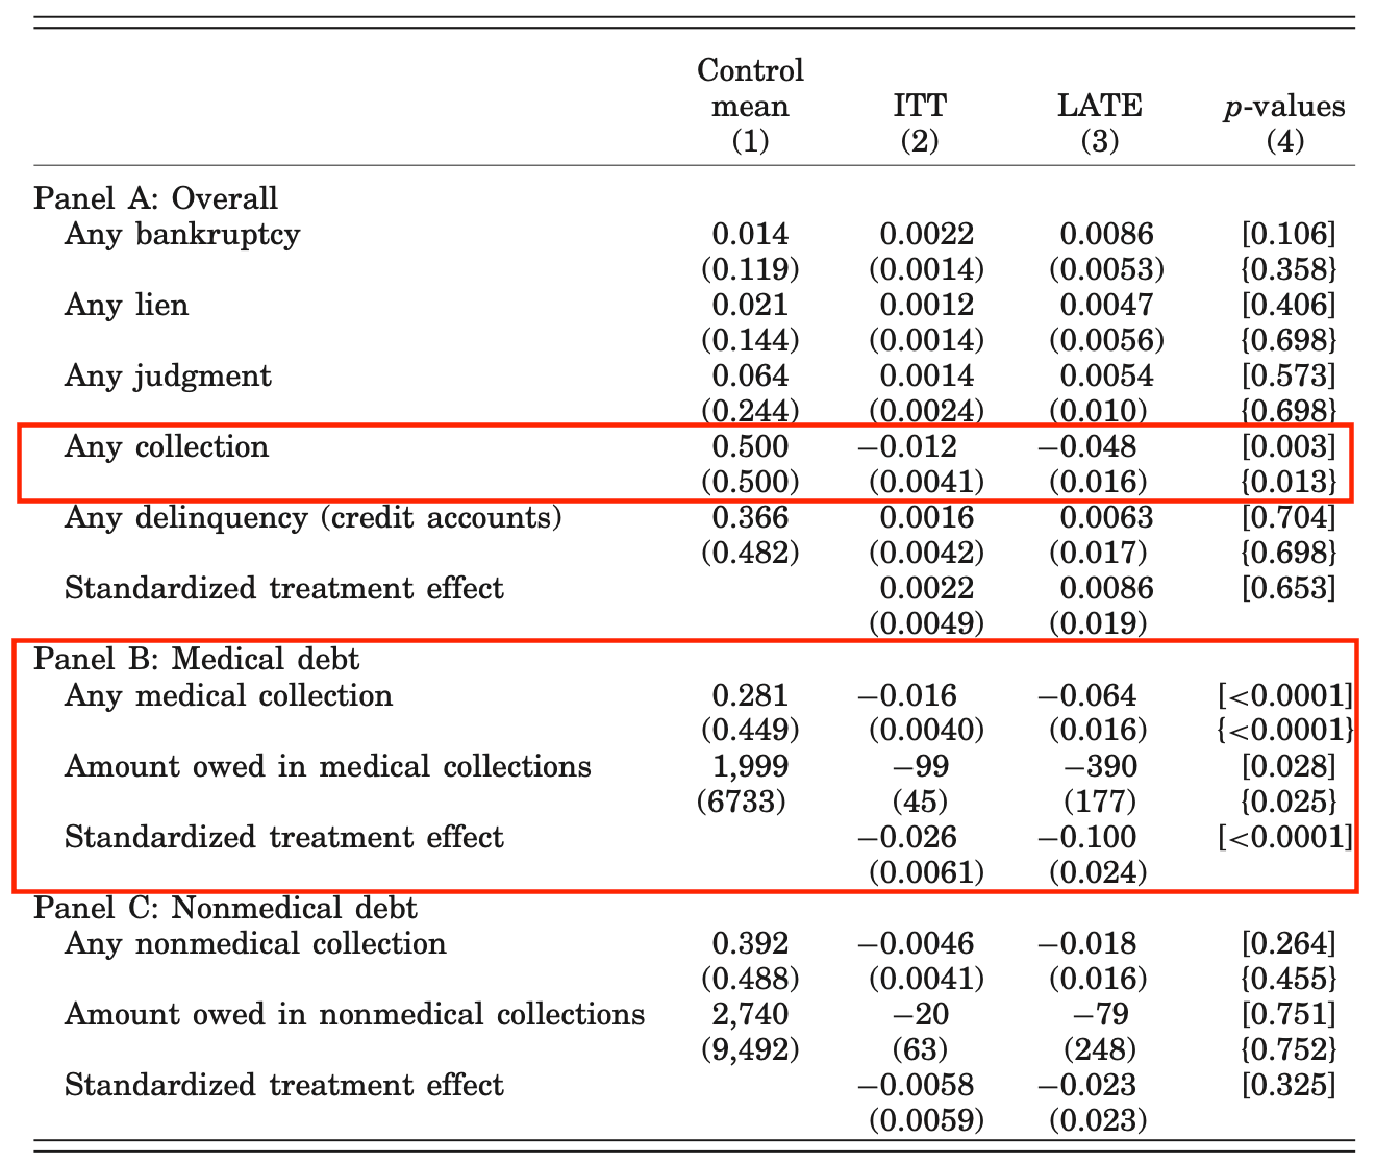
\includegraphics[height=0.85\textheight]{input/ohie_tab7.pdf}
    \end{center}    
    
\end{frame}
%---------------------------------------------------------------------
\begin{frame}{The impact of public insurance on health}
    
    \begin{center}
        \vspace{-3mm}
        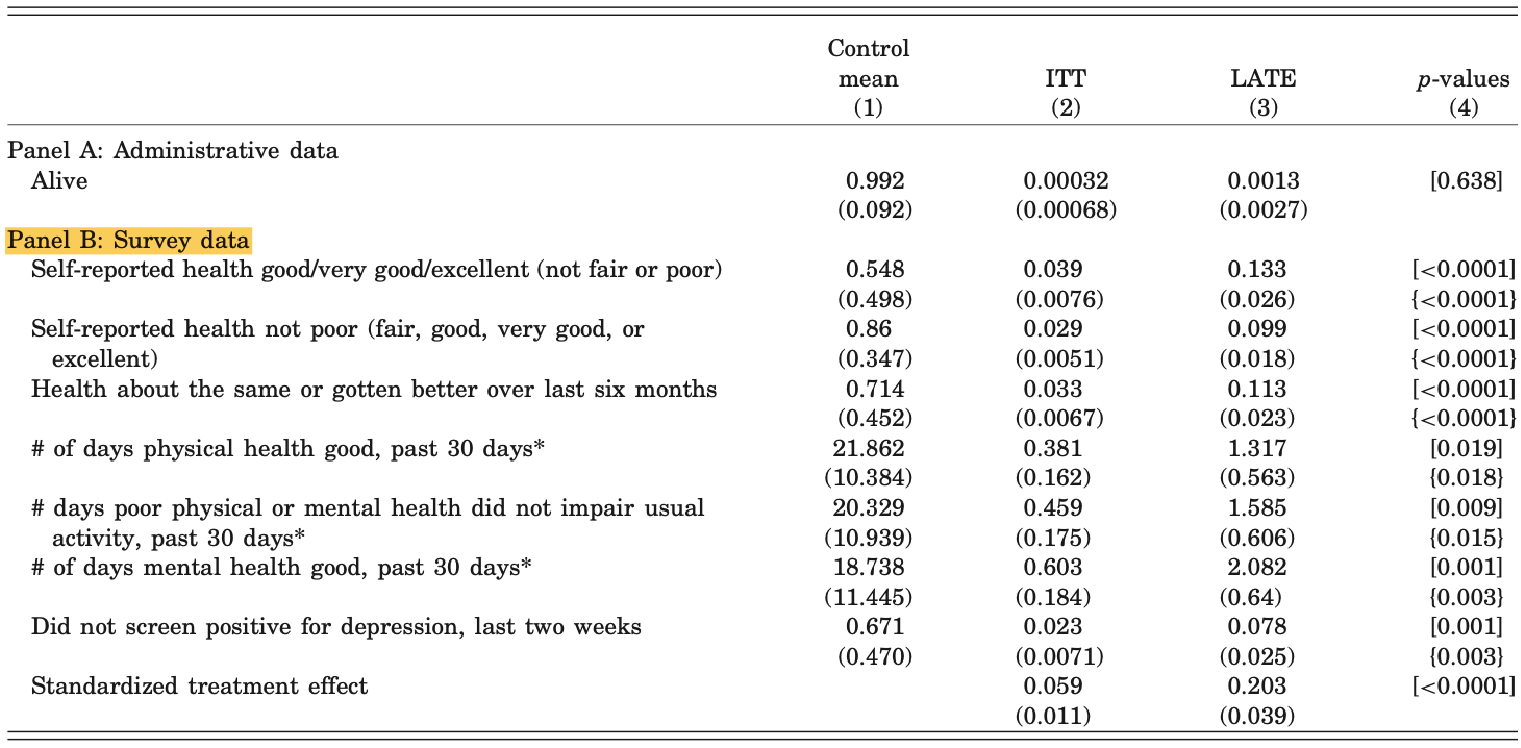
\includegraphics[height=0.8\textheight]{input/ohie_tab9.pdf}
    \end{center}

\end{frame}
%---------------------------------------------------------------------
\begin{frame}{Oregon health insurance experiment: conclusions}
    
        Main findings: \newbold{public insurance}
        \begin{itemize}
            \item Increased healthcare utilization
            \begin{itemize}
                \item No detectable change in ER utilization
                \item Increase in preventive care compliance
            \end{itemize}
            \item Decreased exposure to medical financial liability
            %\\
            %\footnotesize{ \color{gray} See Kluender, Mahoney, Wong, Yin (2024, QJE)} \color{black} \normalsize
            \item Increased health across several self-reported measures
        \end{itemize}
        \vspace{3mm}
    
        Note: these are deeply \newbold{``local''} estimates
        \begin{itemize}
            \item One-year impact of gaining health-insurance
            \item Specific population in a specific time, specific type of public insurance coverage, etc.
        \end{itemize}
        
\end{frame}
%---------------------------------------------------------------------
\begin{frame}{Taking stock}
    % If needed: other evidence of moral hazard: age 65
    % David Card, Carlos Dobkin, and Nicole Maestas

    We have seen that
    \begin{itemize}
        \item Patients respond to prices in healthcare, so that they consume more healthcare when they are insured
        \begin{itemize}
            \item The RAND HIE: higher coinsurance rate $\rightarrow$ lower healthcare utilization
            \item The OHIE: gaining Medicaid insurance increases healthcare utilization
        \end{itemize}
        \item There are benefits to insurance: better health and financial protection
        \begin{itemize}
            \item The OHIE: better self-reported health, more high-value care, better financial health
        \end{itemize}
        \item Higher coinsurance rates reduce both high- and low-value care \dots\\
        $\implies$ Not an ideal tool to curb low-value healthcare spending
    \end{itemize}
    $\implies$ What about \newbold{deductibles}?

\end{frame}
%--------------------------------------------------------------------
\begin{frame}{What about deductibles?}

    \footnotesize\textit{What does a deductible do? The impact of cost-sharing on health care prices, quantities, and spending dynamics.}
    Brot-Goldberg, Chandra, Handel, Kolstad (2017) The Quarterly Journal of Economics
    \normalsize
    \vspace{3mm}

    Taking stock
    \begin{itemize}
        \item There is substantial \newbold{moral hazard} in health insurance
        \item Cost-sharing
        \begin{itemize}
            \item Reduced healthcare utilization
            \item Seemingly \newbold{no impact on health}
        \end{itemize}
    \end{itemize}
    $\implies$ Are deductibles are solution to curb the growth in healthcare spending?
    \vspace{3mm}

    Research question: \newbold{How} are spending reductions achieved with cost-sharing?
        %Are patients curbing on needed healthcare?

\end{frame}
%---------------------------------------------------------------------
\begin{frame}{Setting}

    Data: self-insured large employer
    % primary sample about 76K individuals covered
    \begin{itemize}
        \item Switch from offering both PPO and HDHP to HDHP only
        %Only financial features vary, same network
        \item Ideal population: high income, educated, and technologically savvy
        %high income: no liquidity constraints
        %live close to populated area
    \end{itemize}
    \vspace{5mm}

    \begin{center}
        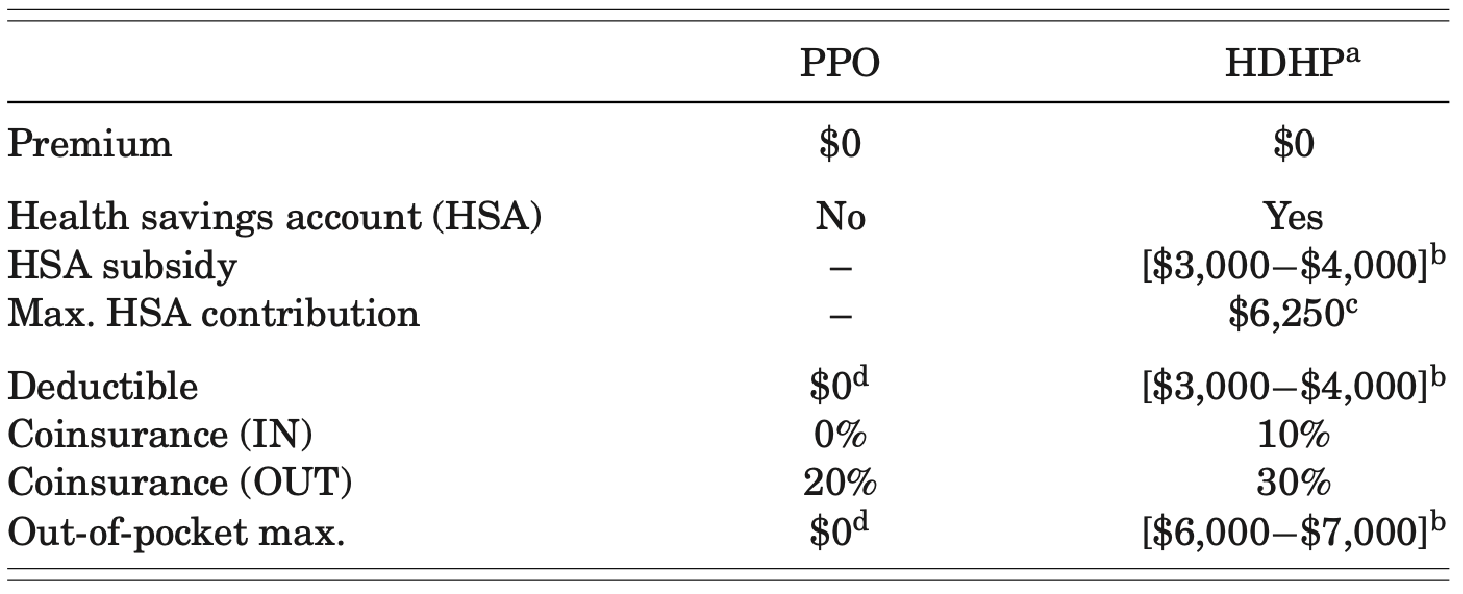
\includegraphics[height=0.55\textheight]{input/BCHK_tab2.pdf}
    \end{center}
%why choosing HDHP? HSA subsidy

\end{frame}
%---------------------------------------------------------------------
\begin{frame}{Healthcare spending changes: time series}
\hypertarget{BCHK:timeseries}{}

    \begin{columns}
        \begin{column}{0.6\textwidth}
            \vspace{-3mm}
            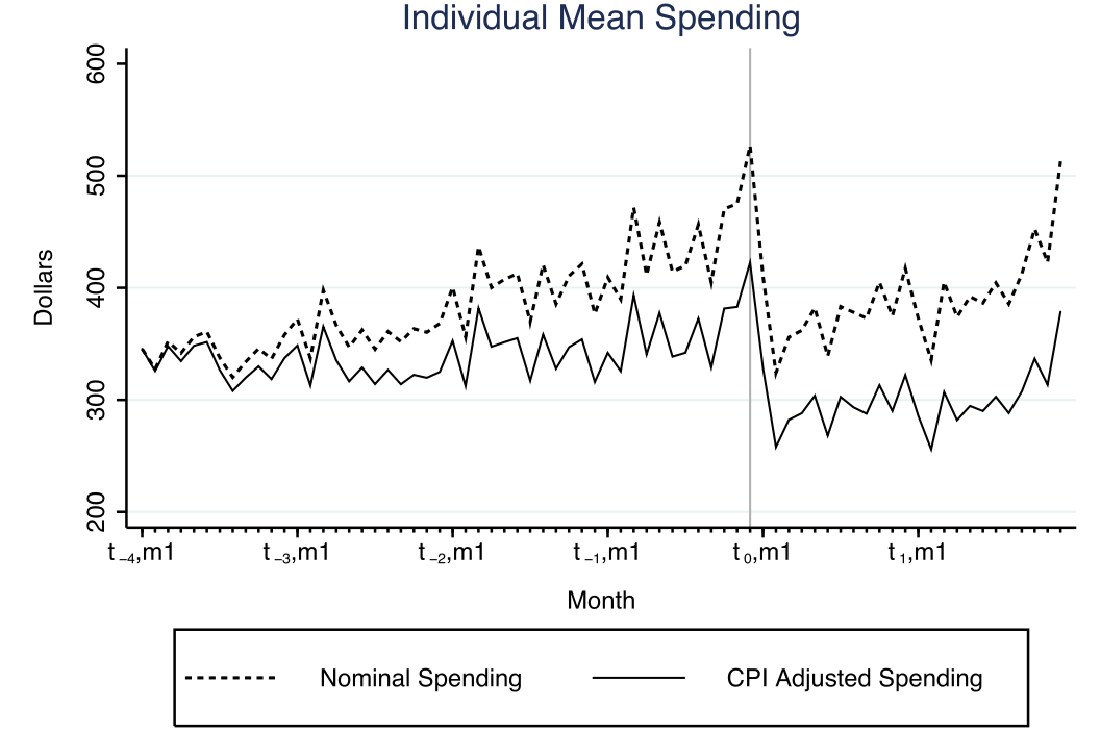
\includegraphics[height=0.7\textheight]{input/BCHK_fig1A.pdf}
        \end{column}
        \begin{column}{0.4\textwidth}
            Necessary adjustments
            \begin{itemize}
                \item Aging
                %regression with age covariates
                \item Price inflation
                %Use Consumer Price Index (CPI)
                %does not adjust for technological changes that woudl lead to higher prices
                \item Anticipatory spending
                %see strategy page 17: regression and use estimates of excess mass (observed over predicted)
                %to adjust the counterfactual observations if no anticipatory spending
            \end{itemize}
            \vspace{5mm}

            %Difference-in-difference results \hyperlink{BCHK:DiD}{\beamergotobutton{}}
        \end{column}
    \end{columns}
\end{frame}
%---------------------------------------------------------------------
\begin{frame}{Healthcare spending changes, by health status}
    
    \begin{center}
        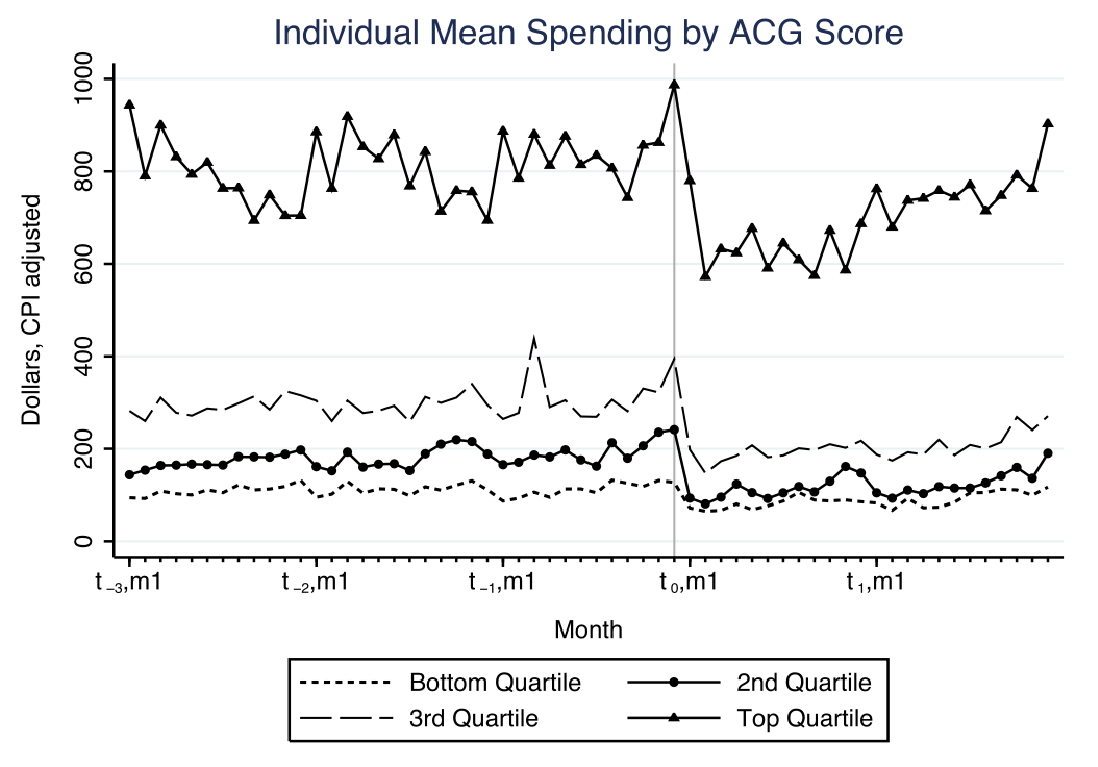
\includegraphics[height=0.8\textheight]{input/BCHK_fig1B.pdf}
    \end{center}
    %ACG score: Johns Hopkins ACG software feed in all healthcare consumption)
    %Shows that sickest reduce the most: not a great sign for "smart" price shopping

\end{frame}
%---------------------------------------------------------------------
\begin{frame}{Decomposition of price changes}
    \hypertarget{BCHK:decomposition}{}

    Total spending change
    \begin{align*}
        \Delta TS_{t+1,t} = \underbrace{\Delta PPI_{t+1,t}}_{\text{Provider price change index}} 
        + \underbrace{\Delta PS_{t+1,t}}_{\text{Price shopping effect}} 
        + \underbrace{\Delta Q_{t+1,t}}_{\text{Quantity changes}} 
        + \underbrace{\Delta QS_{t+1,t}}_{\text{Quantity substitutions}}
    \end{align*}
    \vspace{10mm}


    \hyperlink{BCHK:PS}{\beamergotobutton{Details on price shopping effect}}
    %Note: quantity substitutions are the residuals
\end{frame}
%---------------------------------------------------------------------
\begin{frame}{Decomposition of price changes: results}
    \hypertarget{BCHK:decomposition:results}{}

    \only<1>{
        \begin{center}
            \vspace{-3mm}
            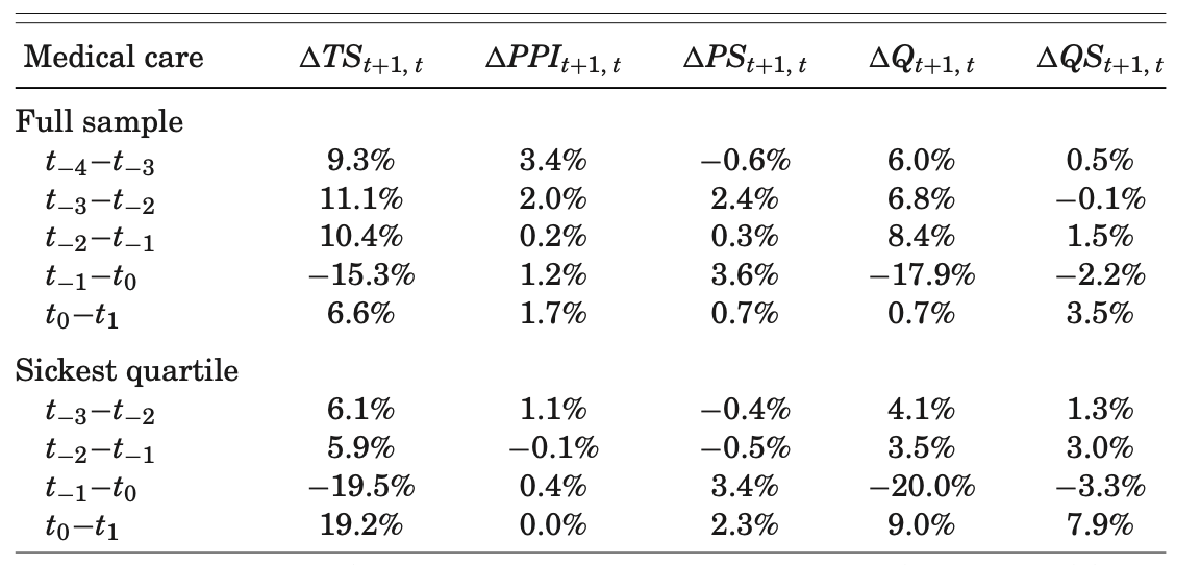
\includegraphics[height=0.8\textheight]{input/BCHK_tab5.pdf}
        \end{center}
    }
    \only<2>{
        \begin{center}
            \vspace{-3mm}
            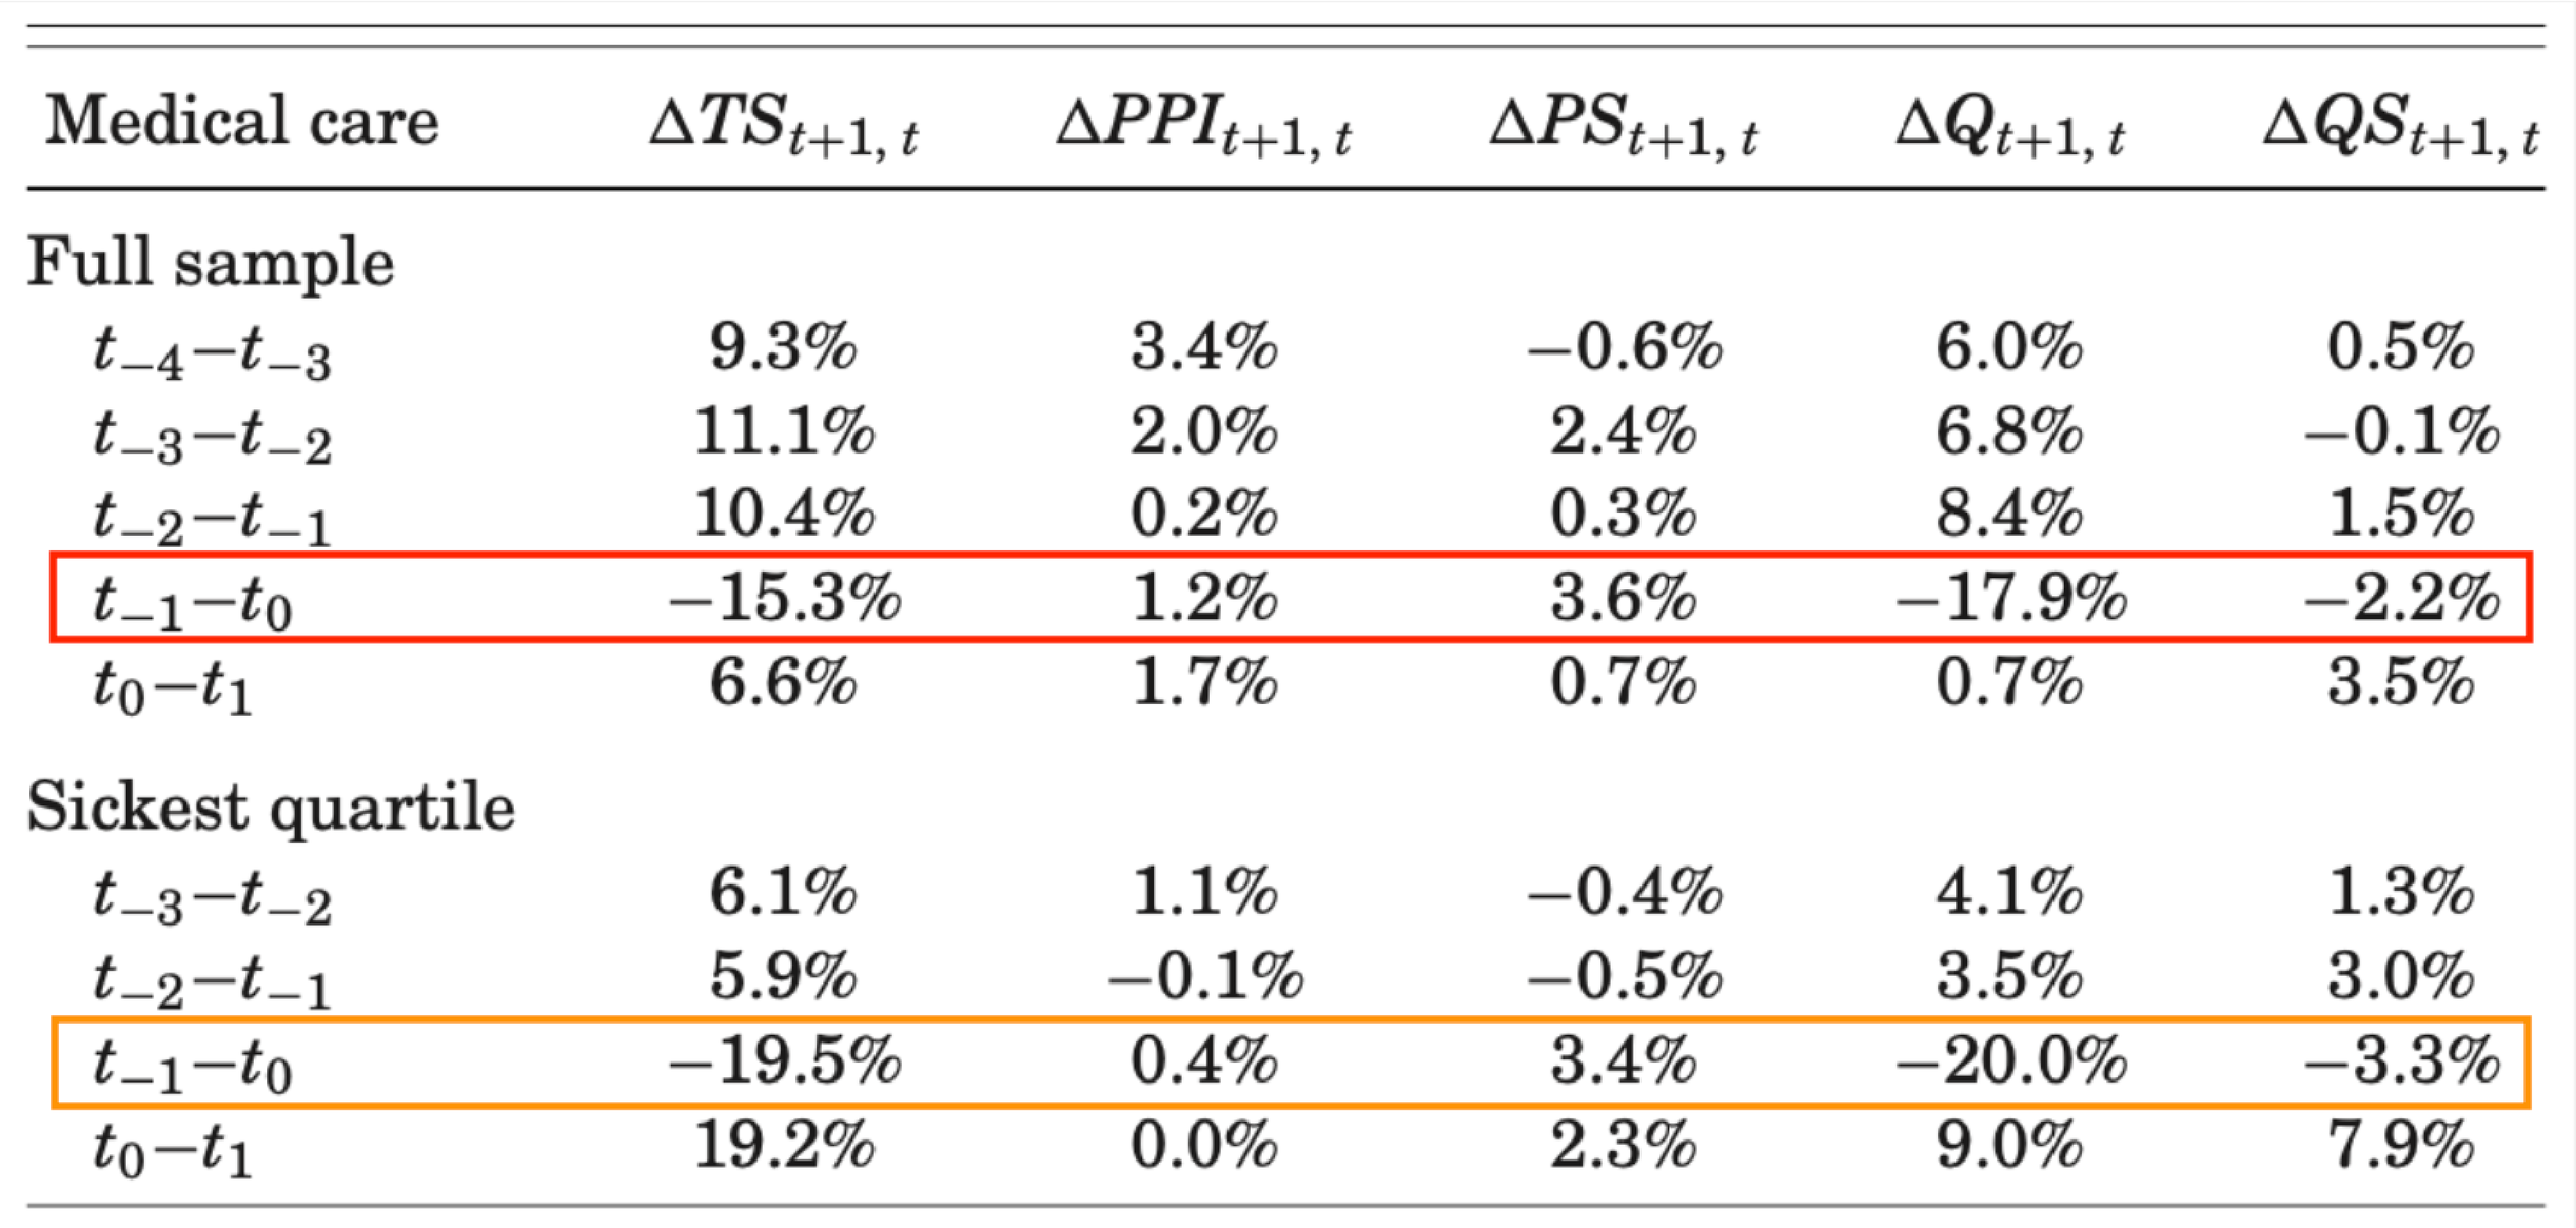
\includegraphics[height=0.8\textheight]{input/BCHK_tab5H.pdf}
        \end{center}
    }

% important things to note:
%(1) there is price shopping, but it does not contribute to the decrease in spending
\end{frame}
%---------------------------------------------------------------------
\begin{frame}{Decomposition of price changes: high-value care}

    \only<1>{
        \begin{center}
            \vspace{-3mm}
            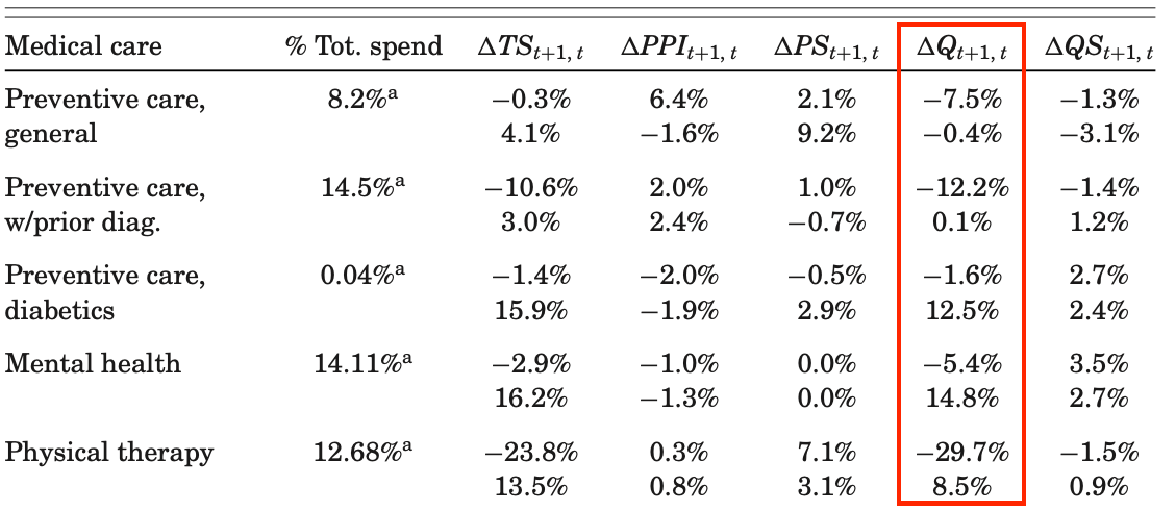
\includegraphics[height=0.7\textheight]{input/BCHK_tab7.pdf}
        \end{center}
    }
    \only<2>{
        \begin{center}
            \vspace{-3mm}
            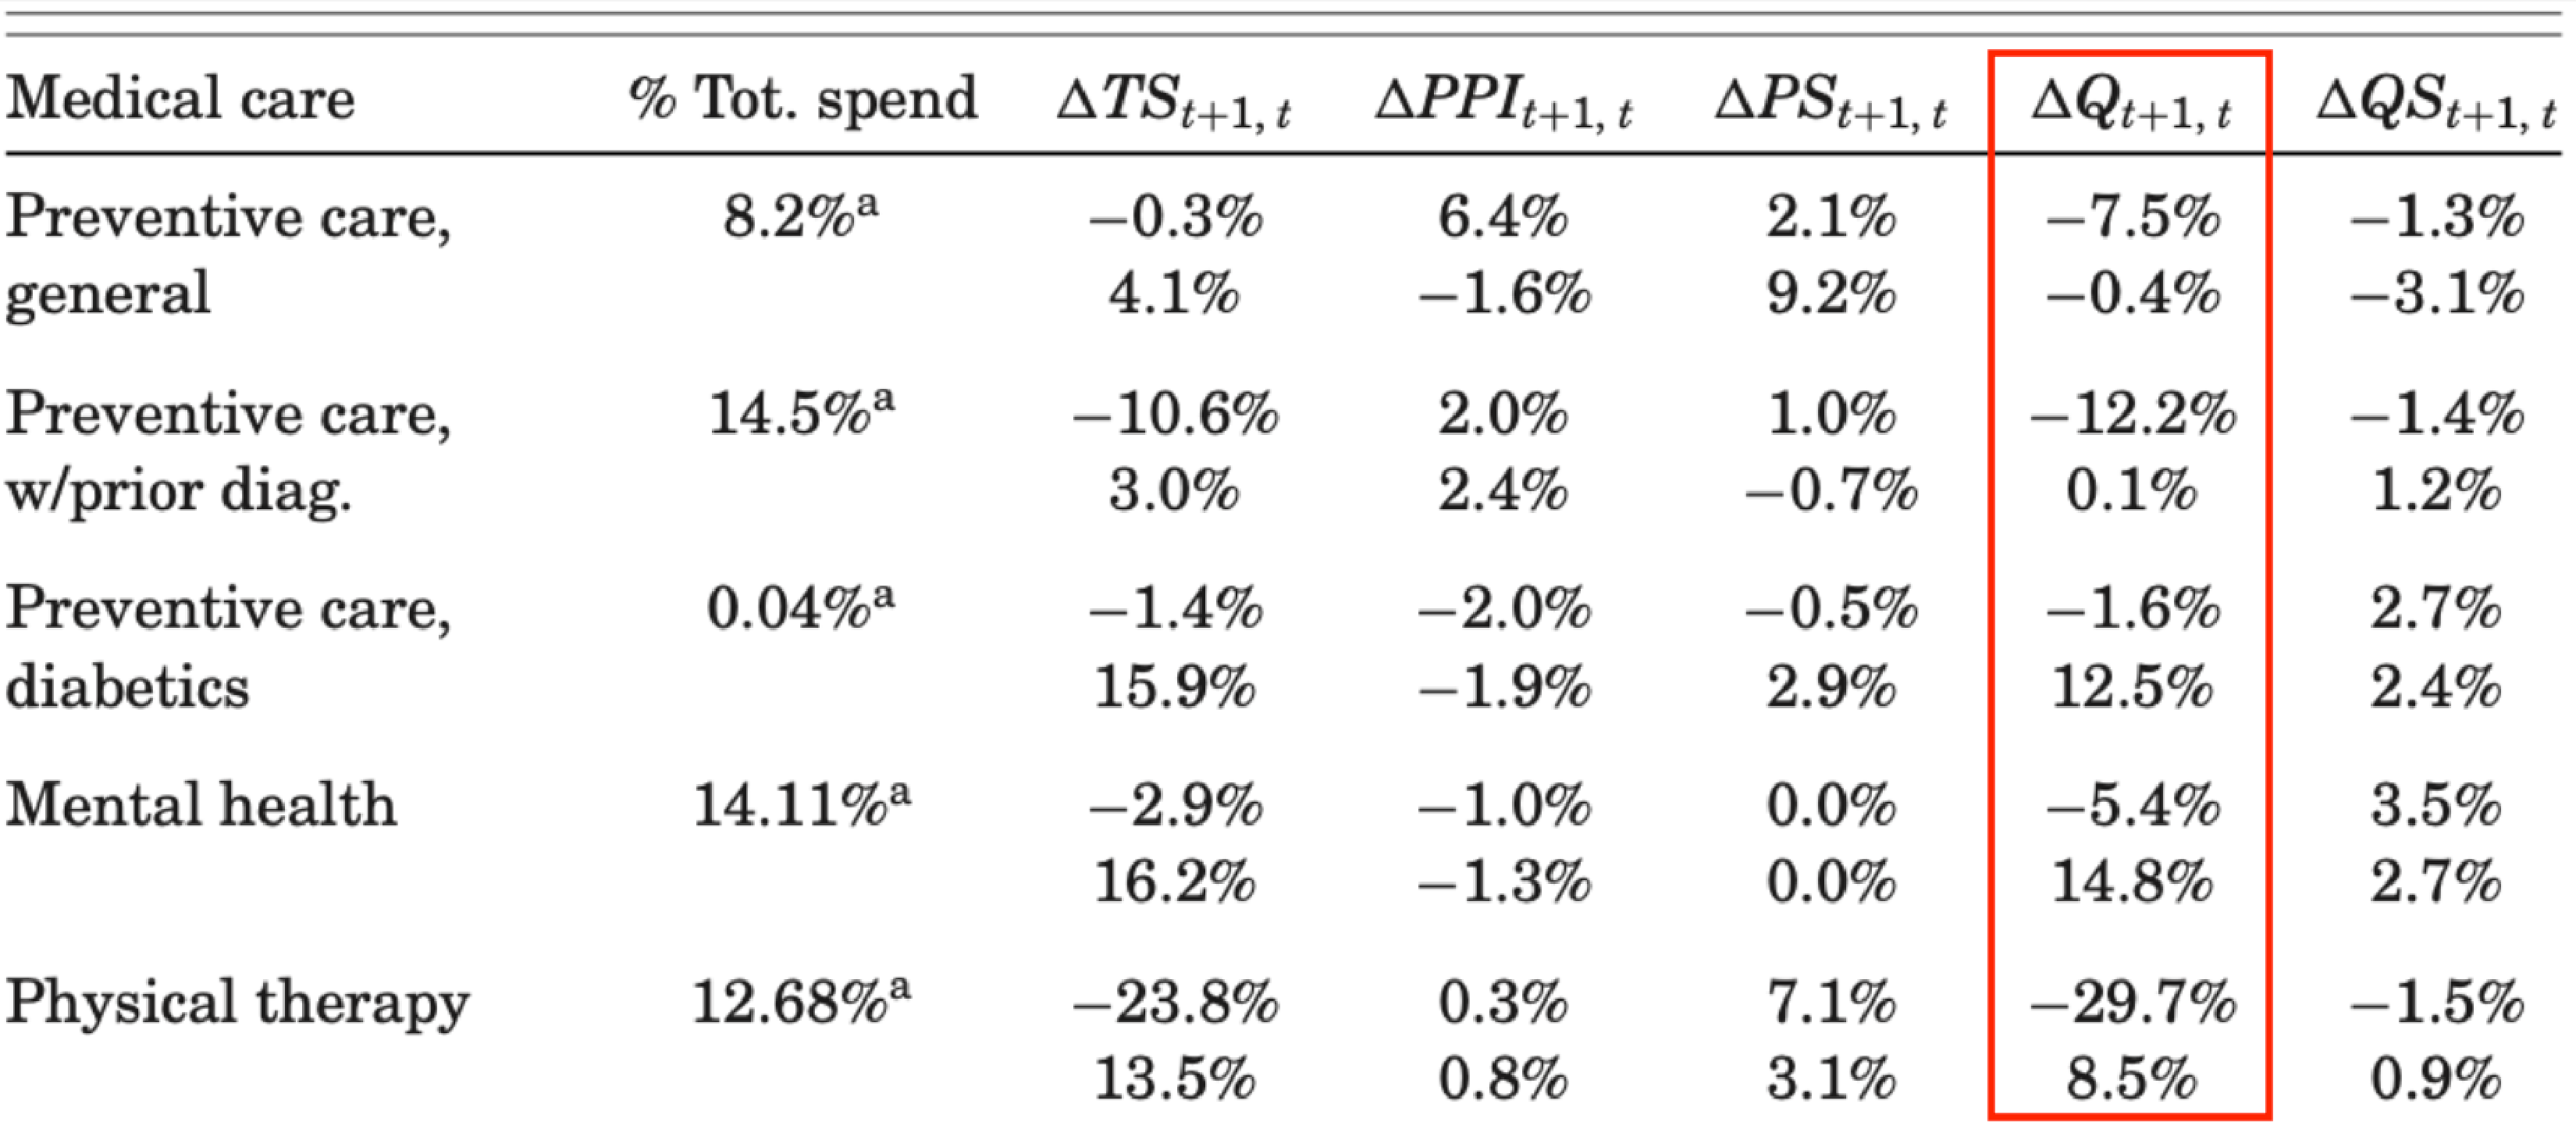
\includegraphics[height=0.7\textheight]{input/BCHK_tab7H.pdf}
        \end{center}
    }
    \only<3>{
        \begin{center}
            \vspace{-3mm}
            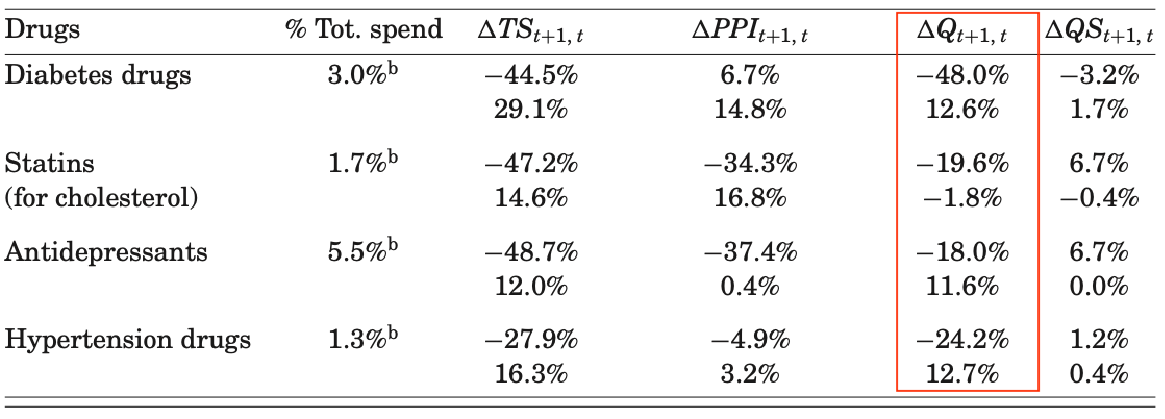
\includegraphics[height=0.6\textheight]{input/BCHK_tab7BH.pdf}
        \end{center}
    }

% Important to note: why reduce free care consumption?
% do not know what is preventive care so free
% preventive care is bundled with more expensive services so if reduce the later reduce both
%See Appendix A9

\end{frame}
%---------------------------------------------------------------------
\begin{frame}{Brief discussion: why reducing free preventive care?}

 Potential explanations for reductions in free preventive care
 \begin{enumerate}
    \item Beneficiaries do not know which care is preventive and hence free
    \item Preventive care is bundled with more expensive services
 \end{enumerate}
%  \vspace{5mm}
 
%  Analyses in Appendix A9: extensive versus intensive margins
%  \begin{itemize}
%     \item Intensive margin: fewer preventive services per primary care visit
%     \item Extensive margin: fewer primary care visits
%  \end{itemize}
%  $\implies$ It is almost all driven by the extensive margin

\end{frame}
%---------------------------------------------------------------------
\begin{frame}{Conclusion: what does a deductible do?}

    How are spending reductions achieved with cost-sharing?
    \begin{itemize}
        \item Reduction in healthcare consumption across the board
        \item Reduce both high-and low-value care
        \item No evidence for increased price shopping
    \end{itemize}
    \vspace{7mm}

    % How do consumers process insurance contracts with non-linearities?
    % \begin{enumerate}
    %     \item Consumers respond more to \newbold{spot prices}
    %     \item Limited evidence for learning
    % \end{enumerate}
    % \vspace{3mm}

    $\implies$ Challenge for \newbold{policy}: reducing spending vs. high-value care consumption


\end{frame}
%---------------------------------------------------------------------
\begin{frame}{Other ways to prevent moral hazard? Prior authorization}

    \newbold{Prior authorization}: health insurers require pre-approval for medical services, procedures, or prescription drugs to ensure they are medically necessary.\\
    \vspace{5mm}

    Debate:
    \begin{itemize}
        \item Increase administrative burden for providers, delays, etc.\\
        $\implies$ administrative costs in healthcare are large: $\sim$ 20 to 34\% of health care expenditures, 1-4\% of GDP
        \item A tool for insurers to fight moral hazard and reduce the use of low value care
        %In healthcare administration, an ordeal refers to a deliberate non-monetary burden imposed on patients as part of accessing care or benefits.
    \end{itemize}

\end{frame}
%---------------------------------------------------------------------
\begin{frame}{Other ways to prevent moral hazard? Prior authorization}

    Prior-authorization in practice
    \begin{itemize}
        \item Form to fill by provider + supportive documentation
        \item Time: 1 to 5 business days
        \item What is restricted: \newbold{drugs}, surgeries, durable medical equipment, imaging
    \end{itemize}
    \vspace{3mm}

    How does it work in theory?
    \begin{itemize}
        \item Information transmission of value to patient
        \item Ordeal: physician willingness-to-pay signals value to patient
    \end{itemize}
    $\implies$ \newbold{``screening ordeal''}

\end{frame}
%---------------------------------------------------------------------
\begin{frame}{Other ways to prevent moral hazard? Prior authorization}

    \vspace{-13mm}

    \begin{center}
        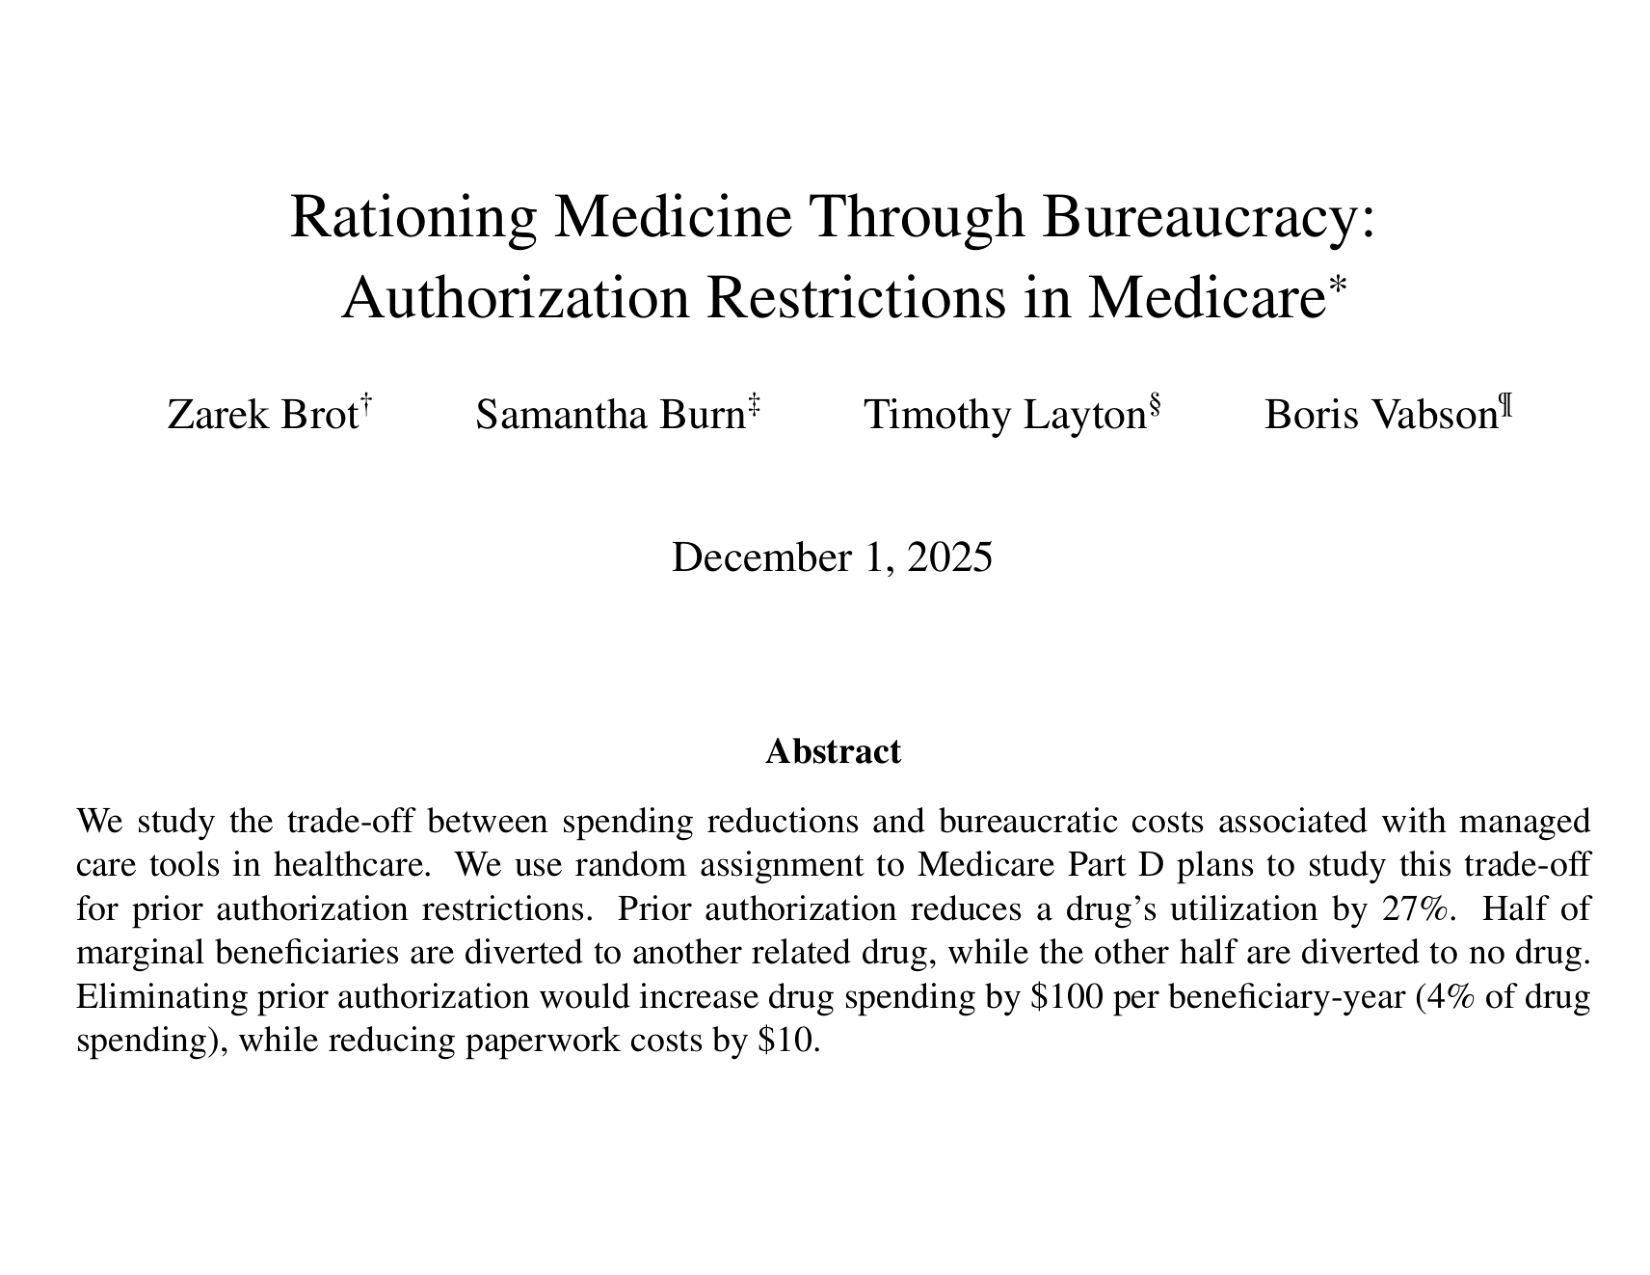
\includegraphics[width=0.8\textwidth]{input/Brotetal2025.pdf}
    \end{center}
    \vspace{-18mm}

    {\scriptsize Brot-Goldberg, Zarek C., Samantha Burn, Timothy Layton, and Boris Vabson. \textit{``Rationing medicine through bureaucracy: authorization restrictions in medicare.''} No. w30878. National Bureau of Economic Research, 2023.}   

\end{frame}
%---------------------------------------------------------------------
\begin{frame}{Example prior authorization form for novel oral anticoagulants (NOACs)}

    \begin{center}
        \vspace{-3mm}
        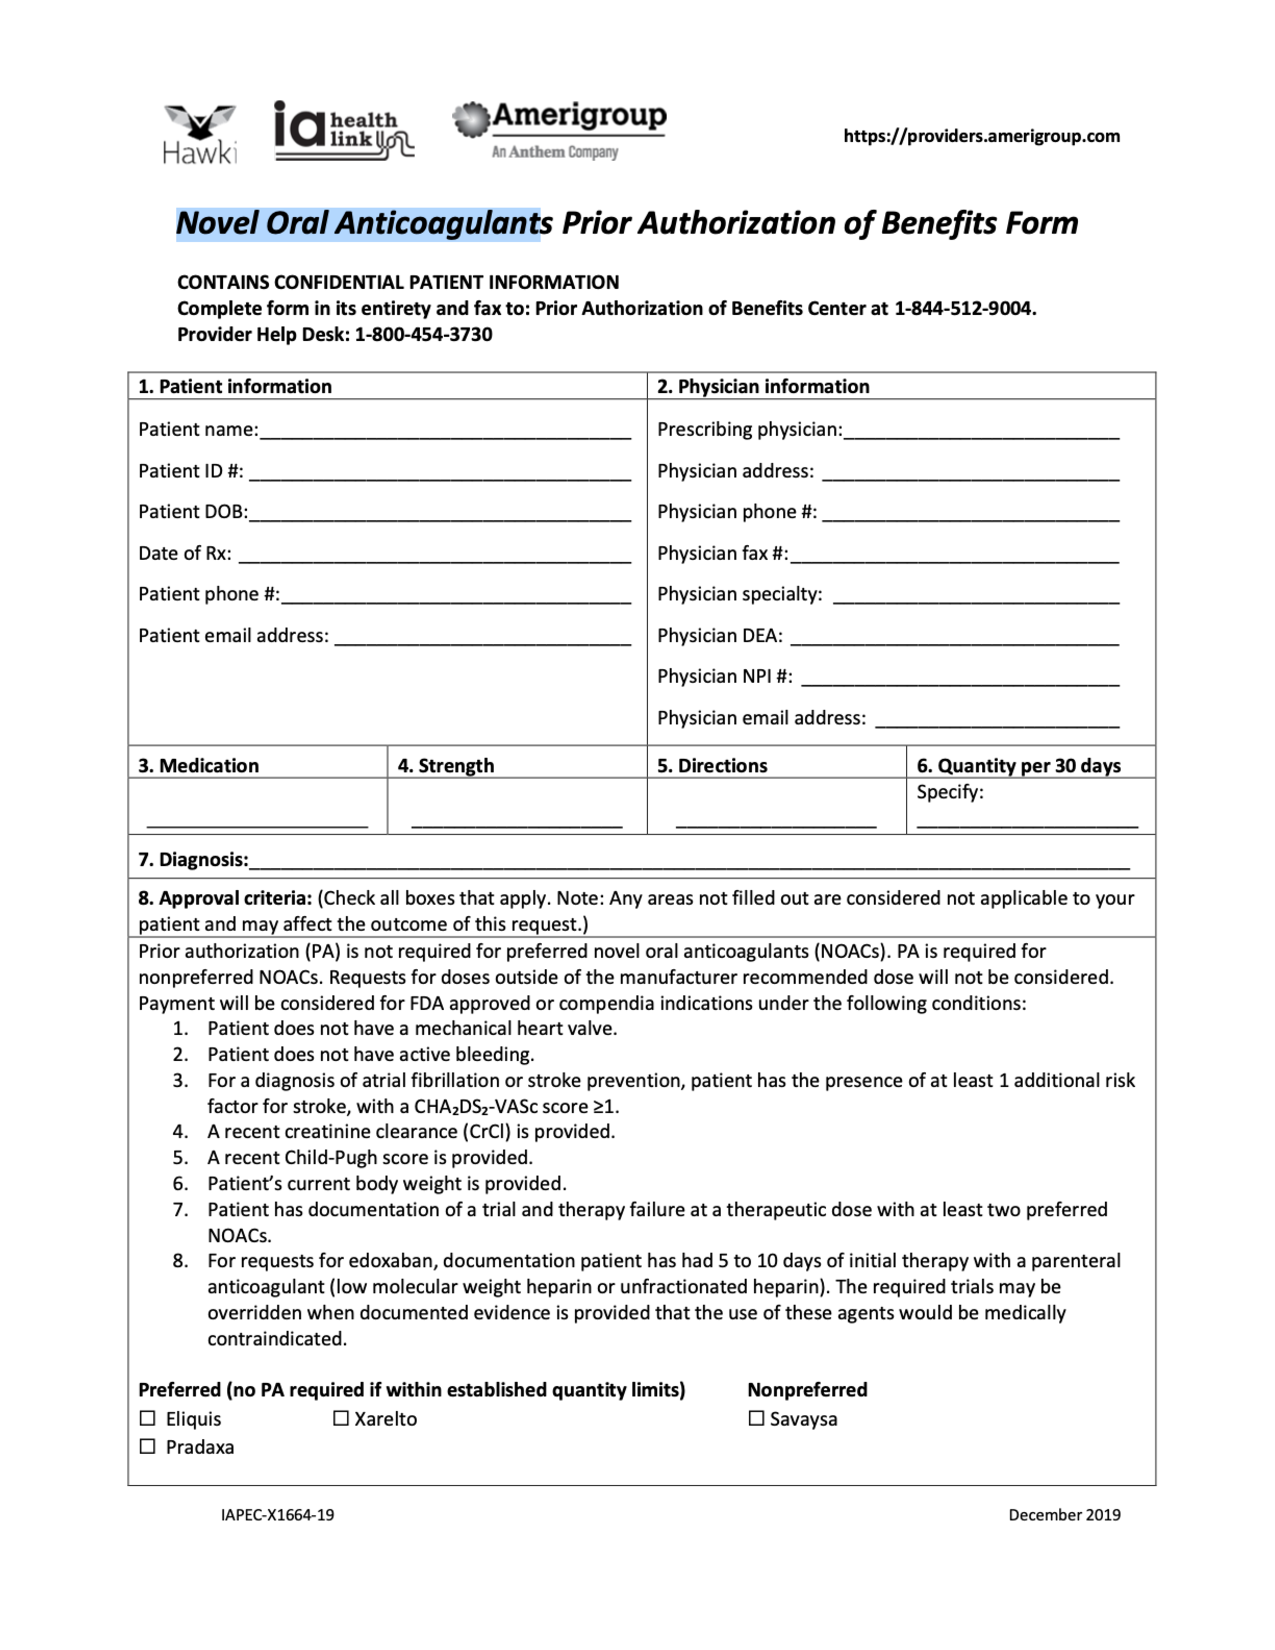
\includegraphics[height=1\textheight]{input/NOACpriorauthform.pdf}
    \end{center}

    % Novel Oral Anticoagulants (NOACs or DOACs) are modern blood-thinners—including apixaban (Eliquis), rivaroxaban (Xarelto), and dabigatran (Pradaxa)—used to prevent stroke and treat blood clots.
    % They are preferred over warfarin for their rapid action, fixed dosing, and lack of required routine blood monitoring.
    % Prior authorization is required to manage their high cost, ensure proper patient selection, and confirm they are used for appropriate indications. 

\end{frame}
%---------------------------------------------------------------------
\begin{frame}{Empirical strategy}

    \newbold{Medicare Part D}: drug insurance (2007-2015)
    \begin{itemize}
        \item Drug insurance component of Medicare, outsourced to private insurers
        \item 34 service regions with a set of plans to choose from
    \end{itemize}
    \vspace{3mm}

    Focus: \newbold{Low income subsidy (LIS)} program
    \begin{itemize}
        \item Offers supplemental financial support
        \item Plans identical in terms of cost-sharing
        \item Differ in drugs covered (substantially)
        \item \newbold{Random default} plan!!
        %\footnotesize Note: data indicates assigned and enrolled plans \normalsize
    \end{itemize}
\end{frame}
%---------------------------------------------------------------------
\begin{frame}{Expensive drugs are more likely to be under prior authorization}

    \begin{center}
        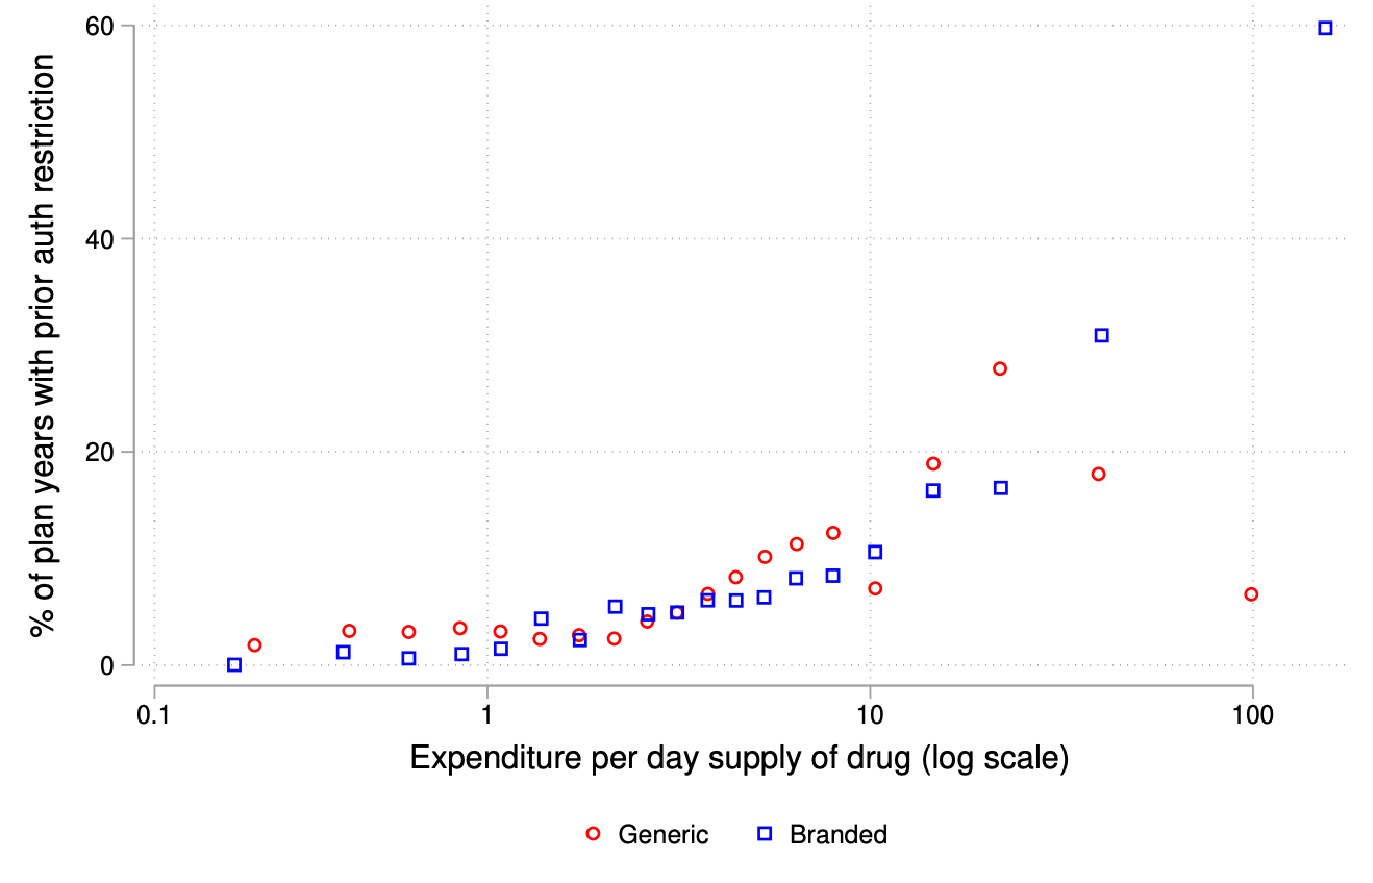
\includegraphics[height=0.8\textheight]{input/BBLV_fig2.pdf}
    \end{center}   

        %top ventile of branded drugs under restriction in 59% of plan years

    
\end{frame}
%---------------------------------------------------------------------
\begin{frame}{Less frequently used drugs are more likely to be under prior authorization}

    \begin{center}
        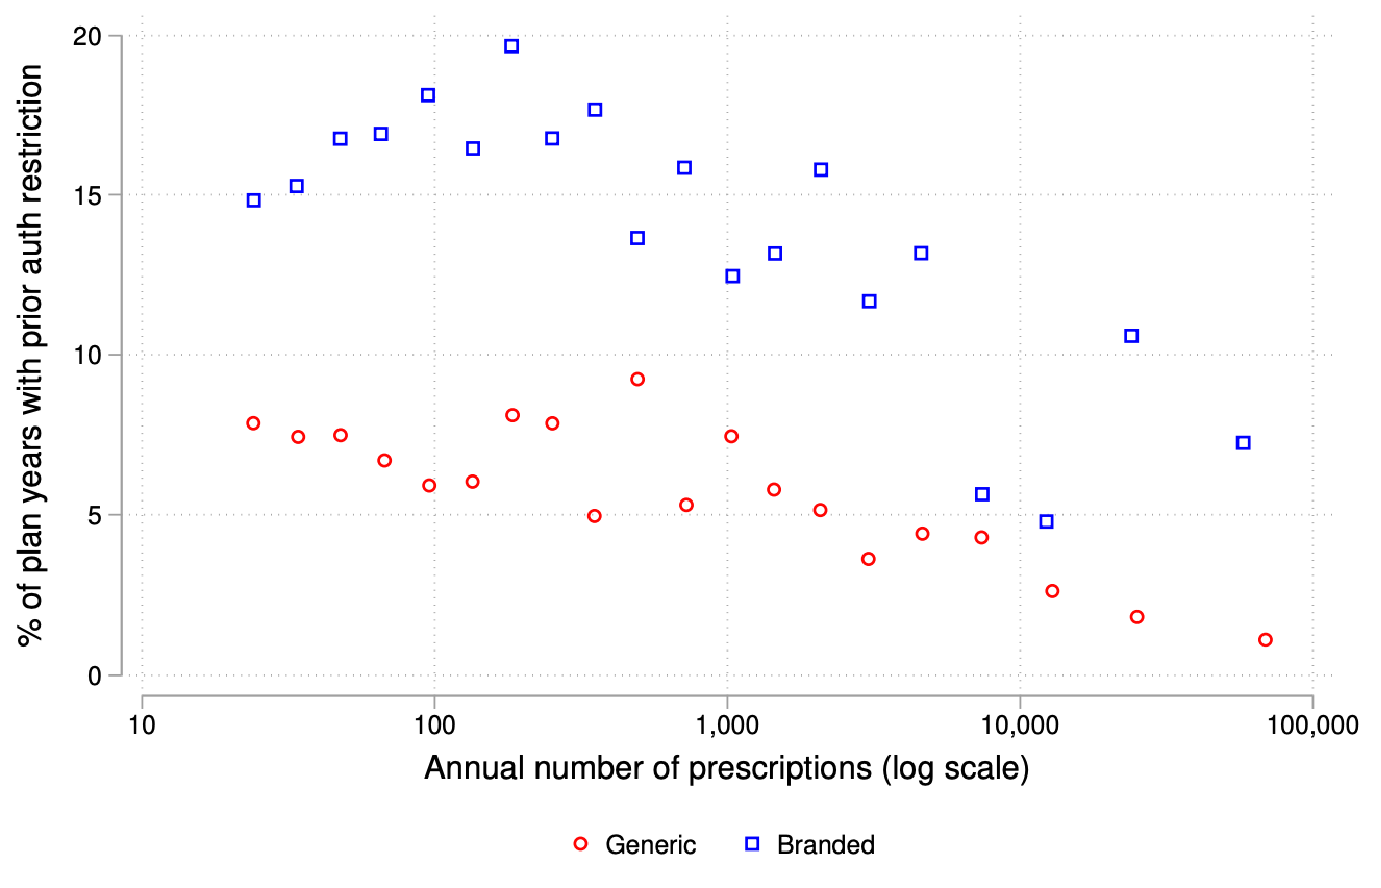
\includegraphics[height=0.8\textheight]{input/BBLV_fig3.pdf}
    \end{center}   

    %conditional on share of beneficiary-years where beneficiary filled the drug at least once
    % less used drugs have less restrictions
    
\end{frame}
%---------------------------------------------------------------------
\begin{frame}{Main take-aways}

    What is the impact of prior authorization on
    \begin{itemize}
        \item \newbold{Financial trade-off}: savings from reduced utilization vs. administrative costs \only<2>{{\color{blue} Produces financial savings}}
        \begin{itemize}
            \item All potential candidates face the administrative costs
            \item Only some candidates will be deterred from using the high-spending treatment
        \end{itemize}
        \item \newbold{Welfare}: impact on patients' consumer surplus \only<2>{{\color{blue} Ambiguous}}
        \begin{itemize}
            \item Who is deterred from using the care: low or high value users?
            \item What treatment get the patients who get denied the treatment? Less expensive treatment, no treatment?
        \end{itemize}
        \item \newbold{Health}: impact on health outcomes \only<2>{{\color{blue} Inconclusive}}
    \end{itemize}

\end{frame}
%---------------------------------------------------------------------
\begin{frame}{Main take-aways (warning)}

    What is the impact of prior authorization on
    \begin{itemize}
        \item \newbold{Financial trade-off}: savings from reduced utilization vs. administrative costs {\color{blue} Produces financial savings}
        \item \newbold{Welfare}: impact on patients' consumer surplus {\color{blue} Ambiguous}
        \item \newbold{Health}: impact on health outcomes {\color{blue} Inconclusive}
    \end{itemize}
    \vspace{5mm}
    These results are \newbold{only for the current menu/design of prior authorization}:\\
    $\implies$ It does not say anything about the impact of expanding prior authorization to other drugs\\
    $\implies$ It \newbold{does NOT mean} we should have prior authorization for all drugs

\end{frame}
%---------------------------------------------------------------------
\begin{frame}{If you want to learn more}

Some of the bureaucracy in health care is ``useful''
\begin{itemize}
    \item Prior-authorization: leads to financial savings and may be welfare enhancing\\
    {\scriptsize \color{gray} Brot-Goldberg, Zarek C., Samantha Burn, Timothy Layton, and Boris Vabson. \textit{``Rationing medicine through bureaucracy: authorization restrictions in medicare.''} No. w30878. National Bureau of Economic Research, 2023.
    \color{black}}
    \item Monitoring led to savings
    {\scriptsize \color{gray} Shi, Maggie. \textit{``Monitoring for waste: Evidence from medicare audits.''} The Quarterly Journal of Economics 139, no. 2 (2024): 993-1049.
    \color{black}}
\end{itemize}

Bureaucracy creates administrative frictions
\begin{itemize}
    \item Claim denials
    {\scriptsize \color{gray} Dunn, Abe, Joshua D. Gottlieb, Adam Hale Shapiro, Daniel J. Sonnenstuhl, and Pietro Tebaldi. \textit{``A denial a day keeps the doctor away.''} The Quarterly Journal of Economics 139, no. 1 (2024): 187-233.
    \color{black}}
\end{itemize}

Checkout \href{https://bfi.uchicago.edu/insights/the-economics-of-health-insurance-denials-pre-authorizations-and-cost-control/}{this} BFI podcast on these three papers!
\end{frame}
%---------------------------------------------------------------------
\begin{frame}{Conclusion}

    Moral hazard in healthcare
    \begin{itemize}
        \item Patients respond to prices in healthcare: \textit{RAND, OHIE}
        \item However, higher cost-sharing reduces both high- and low-value care 
        \begin{itemize}
            \item For coinsurance: \textit{RAND HIE}
            \item For deductibles: \textit{Brot-Goldberg et al., 2017}
        \end{itemize}
        \item Prior-authorization may be a tool to target low-value care: \textit{Brot-Goldberg et al., 2024}
        \begin{itemize}
            \item The financial gains are positive: reduce more cost savings than it adds in administrative cost
            \item The impact on welfare and health is less clear
        \end{itemize}
        \item Insurance has benefits: compliance with high-value care, self-reported health, financial health
    \end{itemize}
            
\end{frame}
%---------------------------------------------------------------------
\begin{frame}{}
    \begin{center}
    \Large \textcolor{maroon}{ping up}
    \end{center}
\end{frame}
%---------------------------------------------------------------------
\begin{frame}{What we covered today}
    \begin{itemize}
    \item What is the impact of gaining insurance
    \item Other ways to prevent moral hazard (deductibles, prior authorization)
    \item Different empirical approaches to study the impact of insurance and cost-sharing (RCT and natural experiments)
\end{itemize}
\end{frame}
%---------------------------------------------------------------------
\begin{frame}{To next class}
\begin{itemize}
    \item No class next Tuesday 02/17 (Monday schedule)
    \item \newbold{Midterm I} in class next \newbold{Thursday 02/19}
    \begin{itemize}
        \item 1h15min: Part 1 with TFU questions, Part 2 with exercises
        \item \newbold{Bring a calculator!!} Phones are not accepted.
        \item Review problem sets and exercises solved in class
    \end{itemize}
\end{itemize}
\end{frame}
%---------------------------------------------------------------------